\chapter{背景知識}

\section{SSD}\label{s2.1}
\indent
SSD,全名:Solid State Drive,中文:固態硬碟。相較於傳統硬碟 HDD (Hard Disk Drive),SSD 改善了噪音、震動、讀寫速度慢,容易因震動外力等因素而毀損等等的問題;SSD 也不需要在資料分散時,藉由重組硬碟磁區來減少讀取時間。而重點是,SSD作為儲存裝置,還具有這些優點:\cite{SSD}
\begin{itemize}
    \item 存取時間固定,不像 HDD 有不穩定的搜尋時間
    \item 體積較小,適合放在筆記型電腦等行動裝置之中
    \item 少了機械結構,所以不會因機械故障導致毀損
\end{itemize}

而這些都是因為 SSD 採用了 NAND FLASH Memory。\cite{SSDFANS}

\subsection{NAND FLASH Memory}\label{s2.1.1}
\indent
是電子抹除式可程式化唯讀記憶體(Electrically-Erasable Programmable Read-Only Memory,簡稱EEPROM或E2PROM)的其中一種,通常為 SSD、記憶卡、以及隨身碟的主要材料元件,可透過電子方式多次複寫。\\
這種元件的基本單位為 Cell,而依據每個 Cell 可儲存的 bit,可分為:\cite{2014xv}
\begin{itemize}
    \item \textbf{SLC:}Single-level Cell   一個 Cell 存一個位元
    \item \textbf{MLC:}Multi-level Cell    一個 Cell 存兩個位元
    \item \textbf{TLC:}Triple-level Cell   一個 Cell 存三個位元
    \item \textbf{QLC:}Quad-level Cell     一個 Cell 存四個位元
\end{itemize}
不過,所有的 NAND FLASH Memory均具有以下特性:
\begin{itemize}
    \item Asymmertic Program/Erase unit
    \item Erase before write
    \item Limited P/E cycles
\end{itemize}
以下將逐一介紹這些特性。

\subsection{Asymmertic Program/Erase Unit}\label{s2.1.2}
\indent
一個 Page 由多個 Flash Cell 所組成,而數以百計的 Page 會組成一個 Block。\\
而 Asymmertic Program/Erase Unit 指的意思是,當要讀取或是寫入時,可以 Page 為單位寫入,但是如果要 Erase 的時候,一次只能以 Block 為單位,無法以 Page 為單位 Write/Read 跟 Erase 的大小不一樣,所以稱為 Asymmertic (非對稱)。(如圖\ref{f2.1}所示)
\begin{figure}[H]
    \centering
    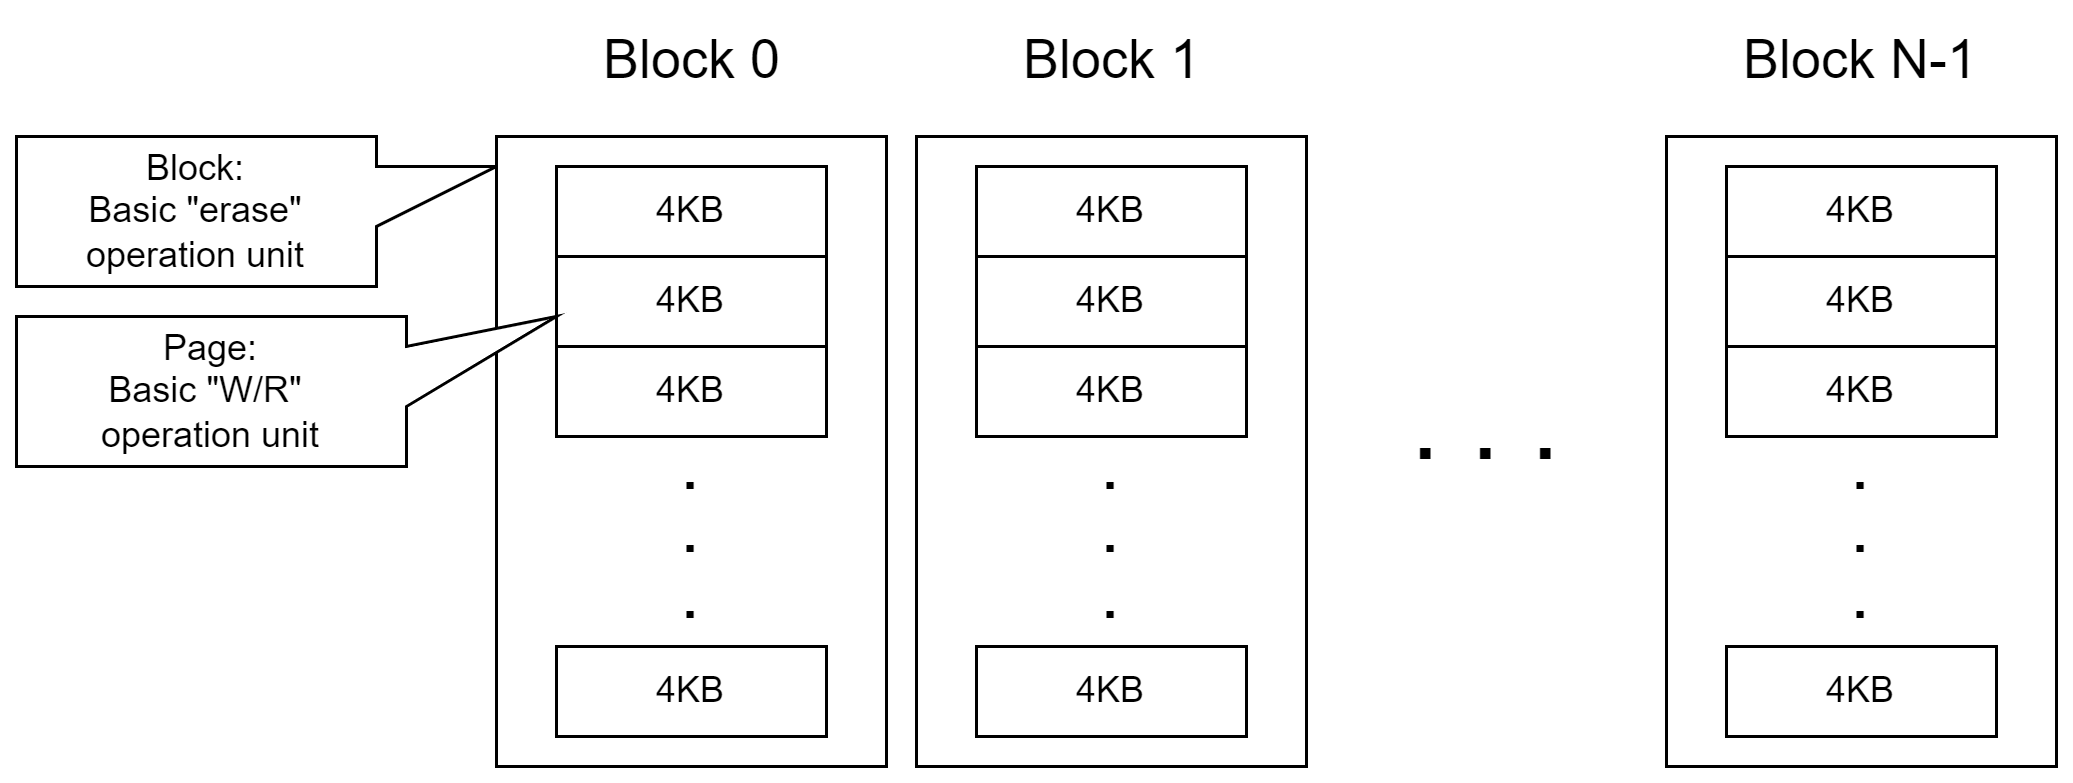
\includegraphics[width=1\textwidth]{picture/ch2/Asymmertic_P-E_unit.png}
    \caption{Asymmertic Program/Erase Unit}
    \label{f2.1}
\end{figure}

\subsection{Erase Before Write}\label{s2.1.3}
\indent
一旦寫入資料到一個 Page 裡面,如果要更改 Page 裡面的資料,只能先清空(Erase),再將資料寫入。而且如\ref{s2.1.2}節所述,清空時只能清空比 Page 還大的 Block 才行。(如圖\ref{f2.2}所示)\cite{SRFTL}
\begin{figure}[H]
    \centering
    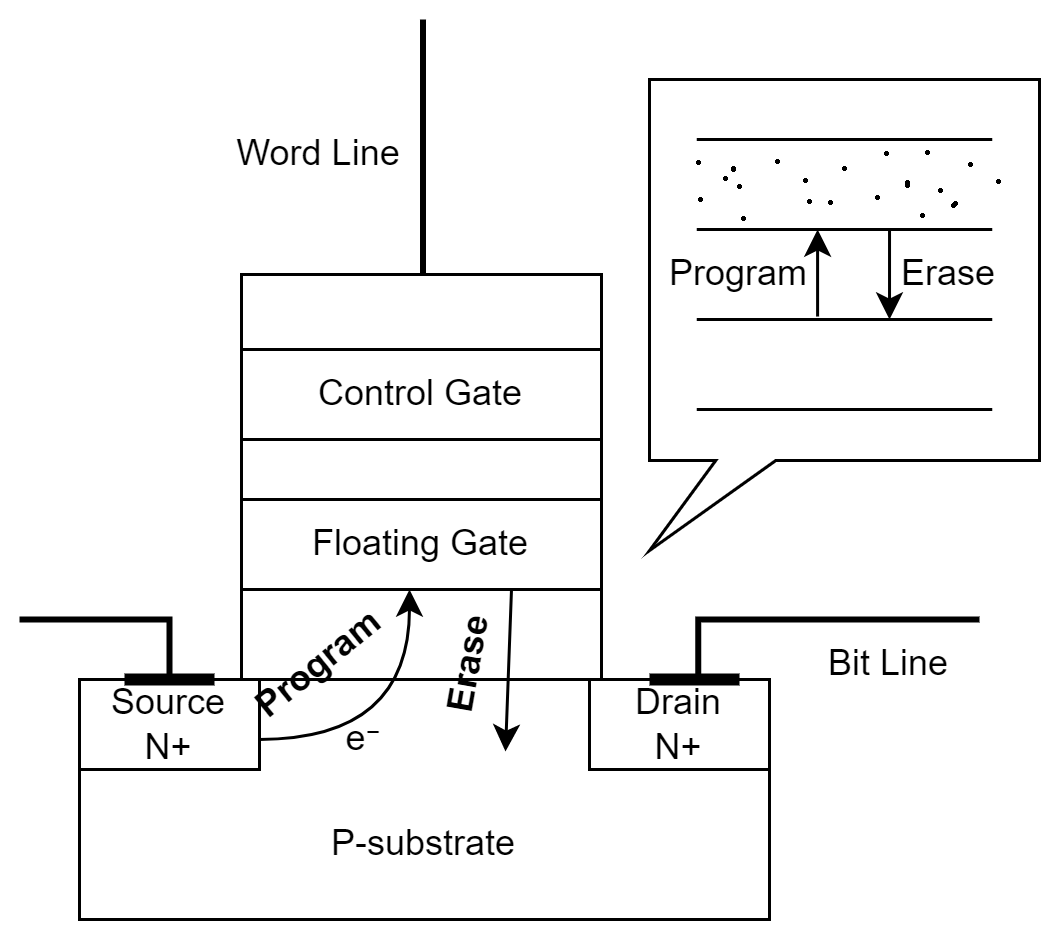
\includegraphics[width=0.6\textwidth]{picture/ch2/erase_before_write.png}
    \caption{Erase Before Write}
    \label{f2.2}
\end{figure}

\subsection{Limited P/E Cycles}\label{s2.1.4}
\indent
Limited Program/Erase Cycle,簡稱Limited P/E Cycle,又被稱為 Wear Out。每次寫入會為用來儲存電子的 Flash Memory Cell 帶來不可逆的損害,原因是每次電子出入 Cell ,Floating Gate 旁邊的 Oxide layer 就會越來越薄(如圖\ref{f2.3}所示),最後因過薄導致無法鎖住電子,整個 Cell 就會毀損\cite{8631191}。而隨著 Flash Memory 的製造商想要把越多的位元塞進一個 Cell 裡面,這些 Cell 的壽命就越來越少,例如 MLC,TLC,QLC 等等。
\begin{figure}[H]
    \centering
    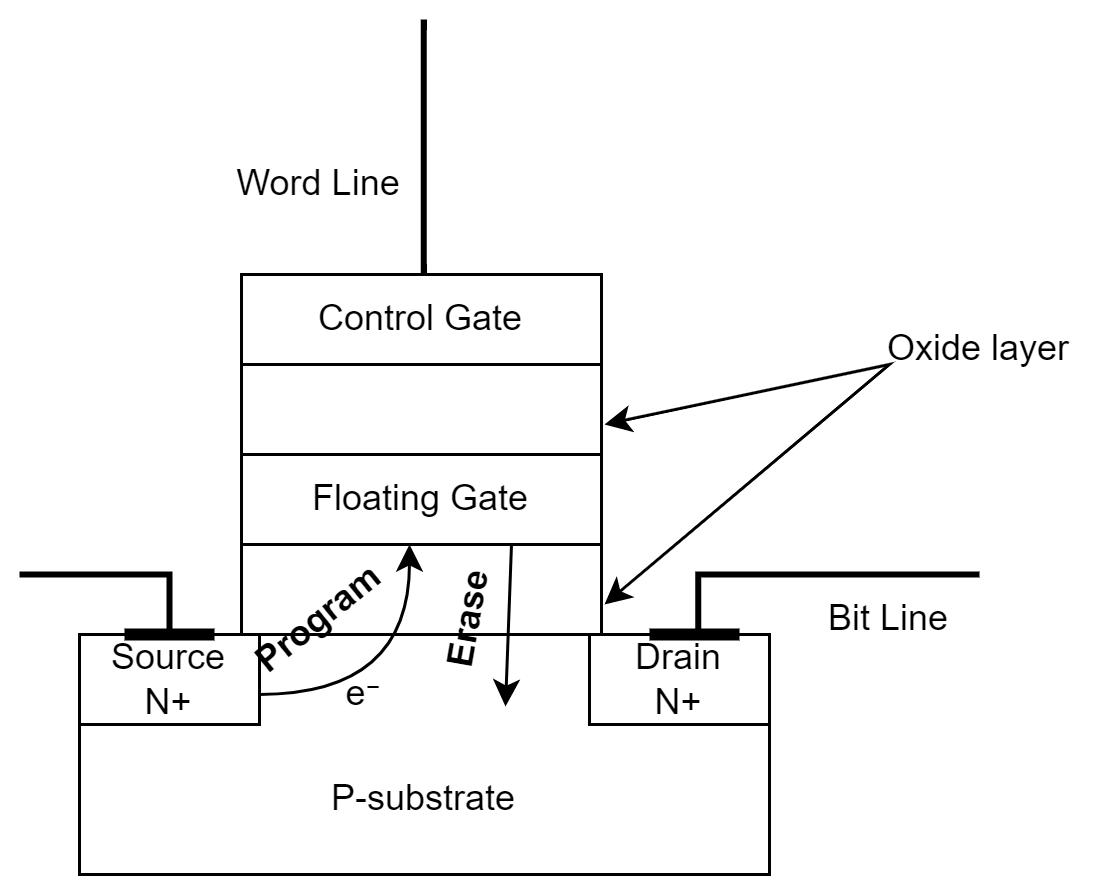
\includegraphics[width=0.6\textwidth]{picture/ch2/Limited_P-E_Cycles.png}
    \caption{Limited P/E cycles}
    \label{f2.3}
\end{figure}

\section{FTL}\label{s2.2}
\indent
為了降低\ref{s2.1.2}節至\ref{s2.1.4}節所提到的特性造成壽命銳減的問題,SSD的製造商通常都會將 FTL 導入至 SSD 裡面(如圖\ref{f2.4}所示)。
FTL 的全名為 Flash Translation Layer,負責針對 Flash Memory 特性而產生的技術,並模擬成一個普通的硬碟,讓作業系統管理SSD與傳統硬碟 (HDD) 的方式一致。而其中的技術通常包含:\cite{Boukhobza2014ASA}
\begin{itemize}
    \item Wear Leveling
    \item Mapping Table
    \item Garbage Collection
\end{itemize}
\begin{figure}[H]
    \centering
    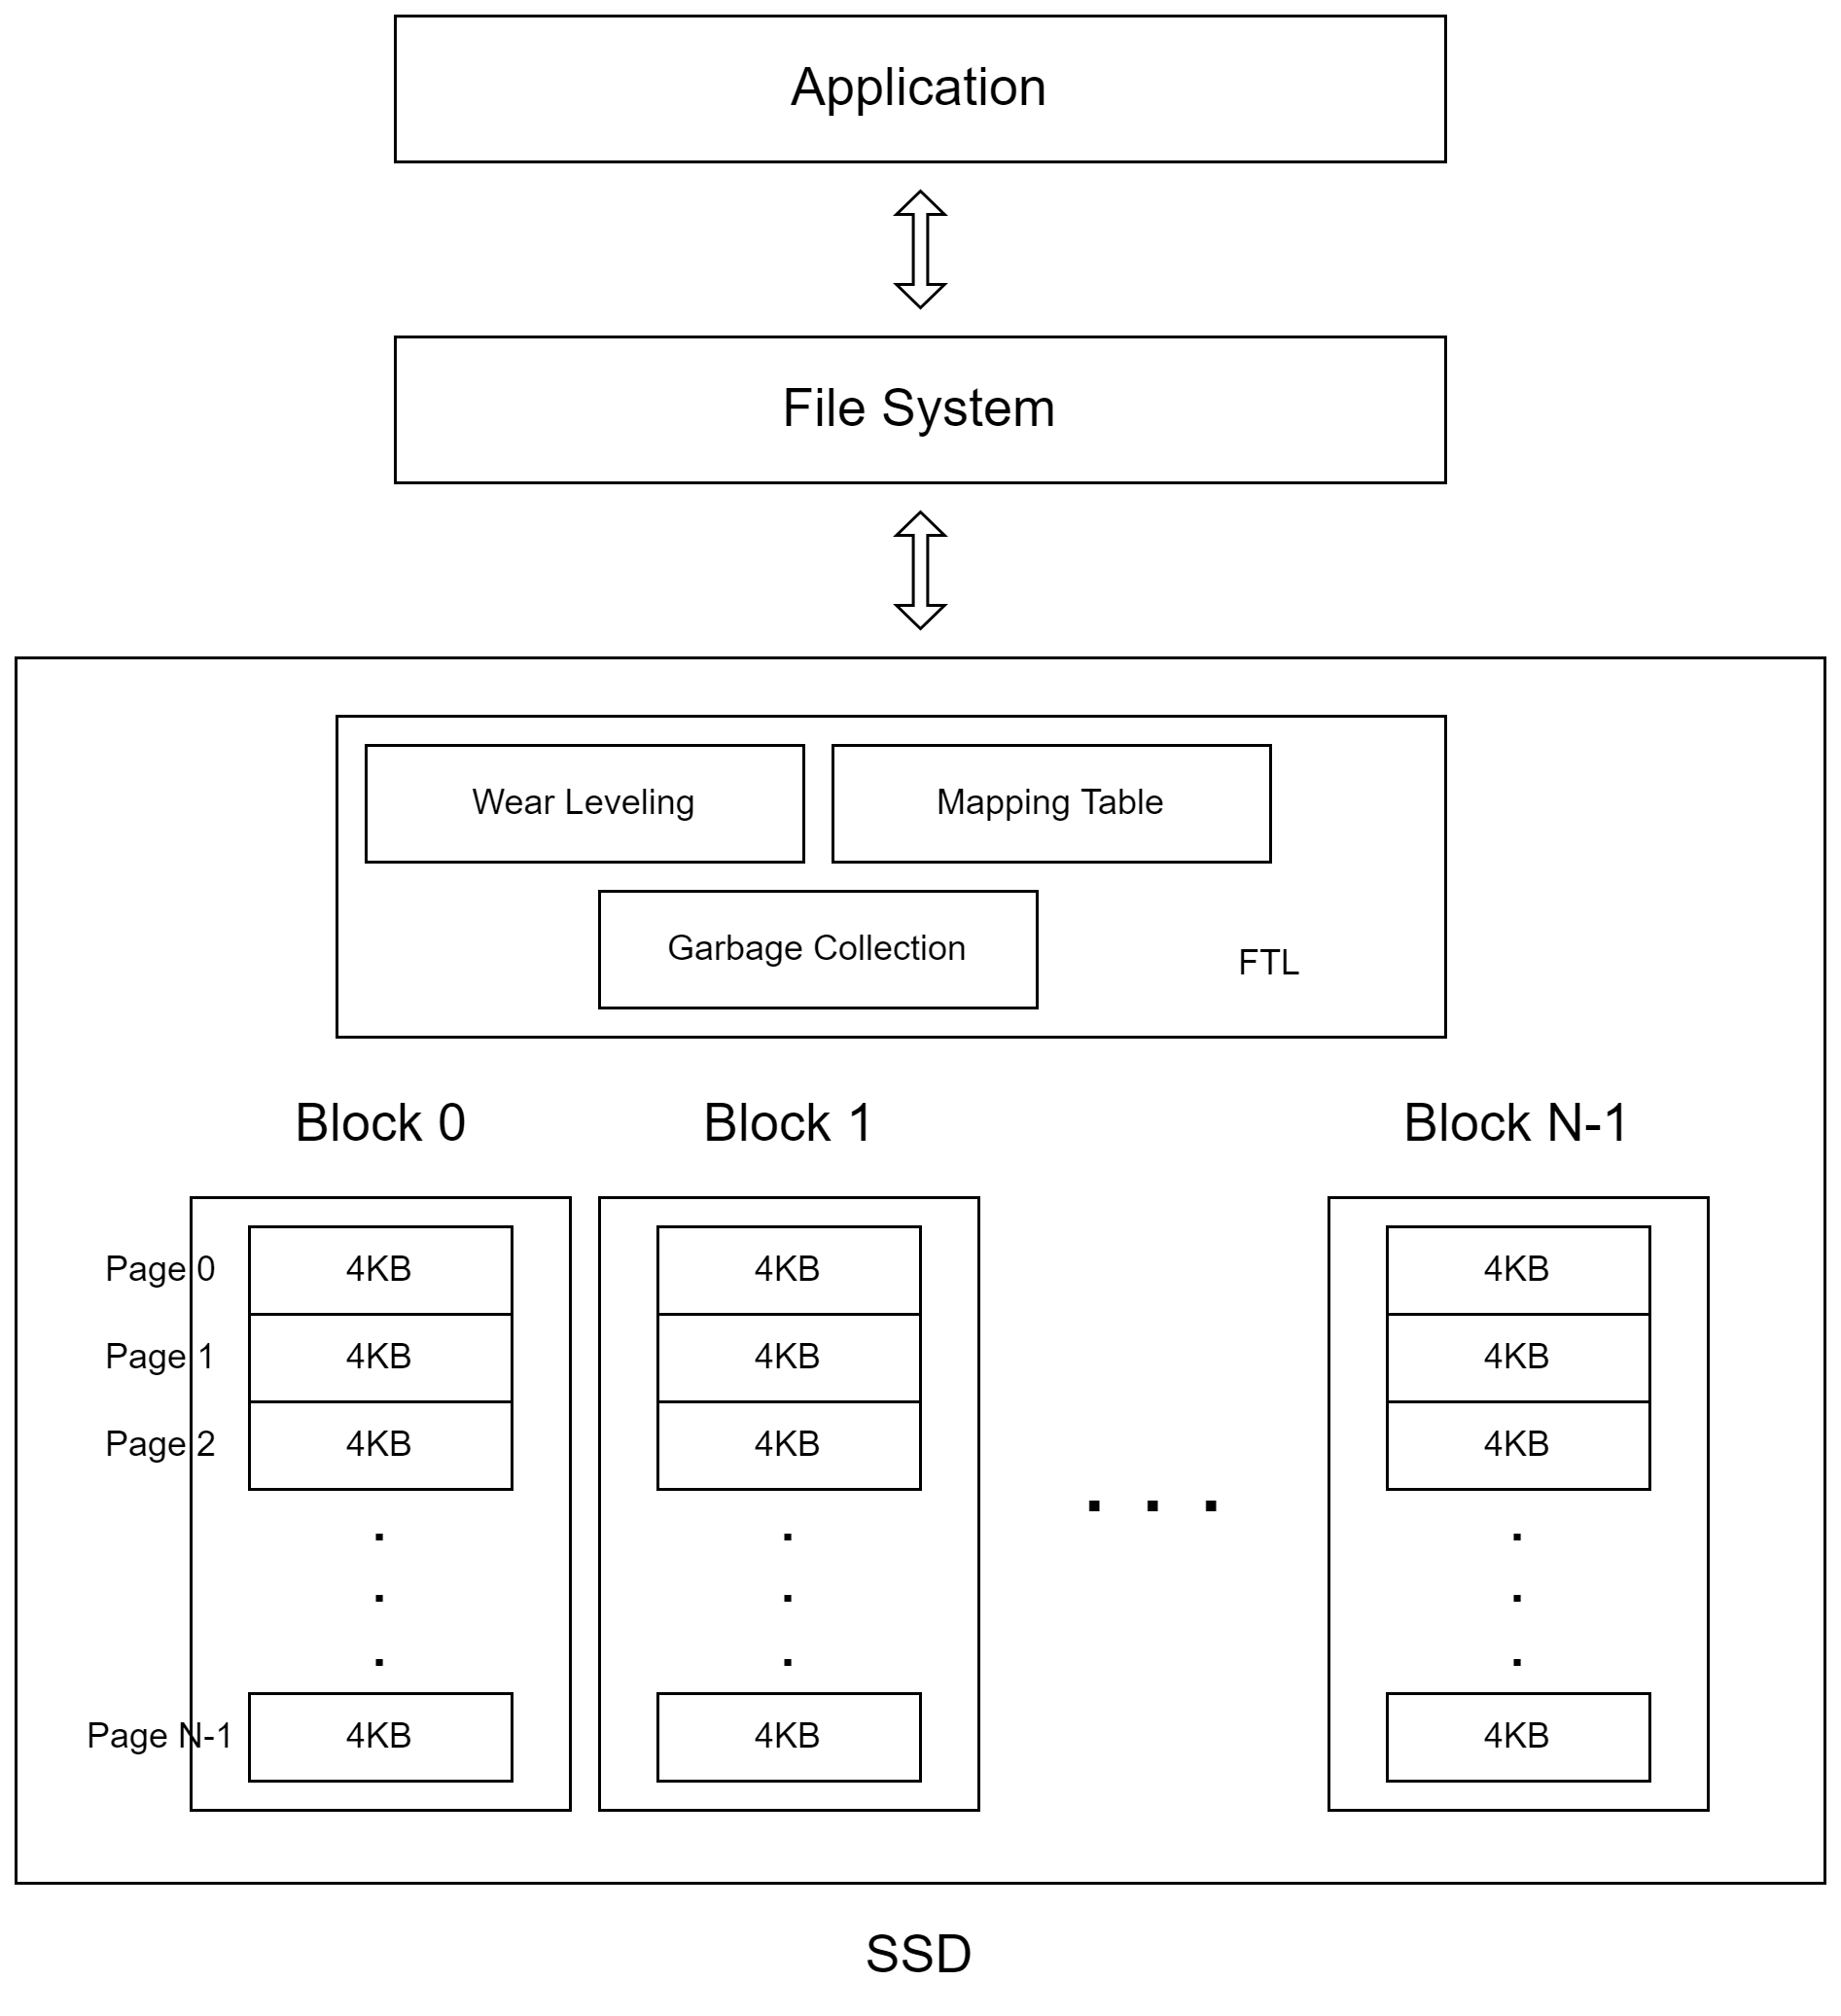
\includegraphics[width=0.8\textwidth]{picture/ch2/FTL.png}
    \caption{Flash Translation Layer}
    \label{f2.4}
\end{figure}
以下將逐一介紹這些技術。

\subsection{Wear Leveling}\label{s2.2.1}
\indent
因為\ref{s2.1.4}節所提到的問題,如果每次都寫入同一個位置會導致 Cell 的壽命大幅衰減,因此為了延長每個 Cell 的壽命,寫入時需要從壽命比較長的 Cell,也就是當下寫入次數較少的 Cell 開始寫入,以平均整體 SSD 的壽命(如圖\ref{f2.5}所示)。所以 SSD 會記錄每個 Cell 的存取次數,來決定下次要寫入到哪裡。\cite{Wear_Leveling_Thesis}
\begin{figure}[H]
    \centering
    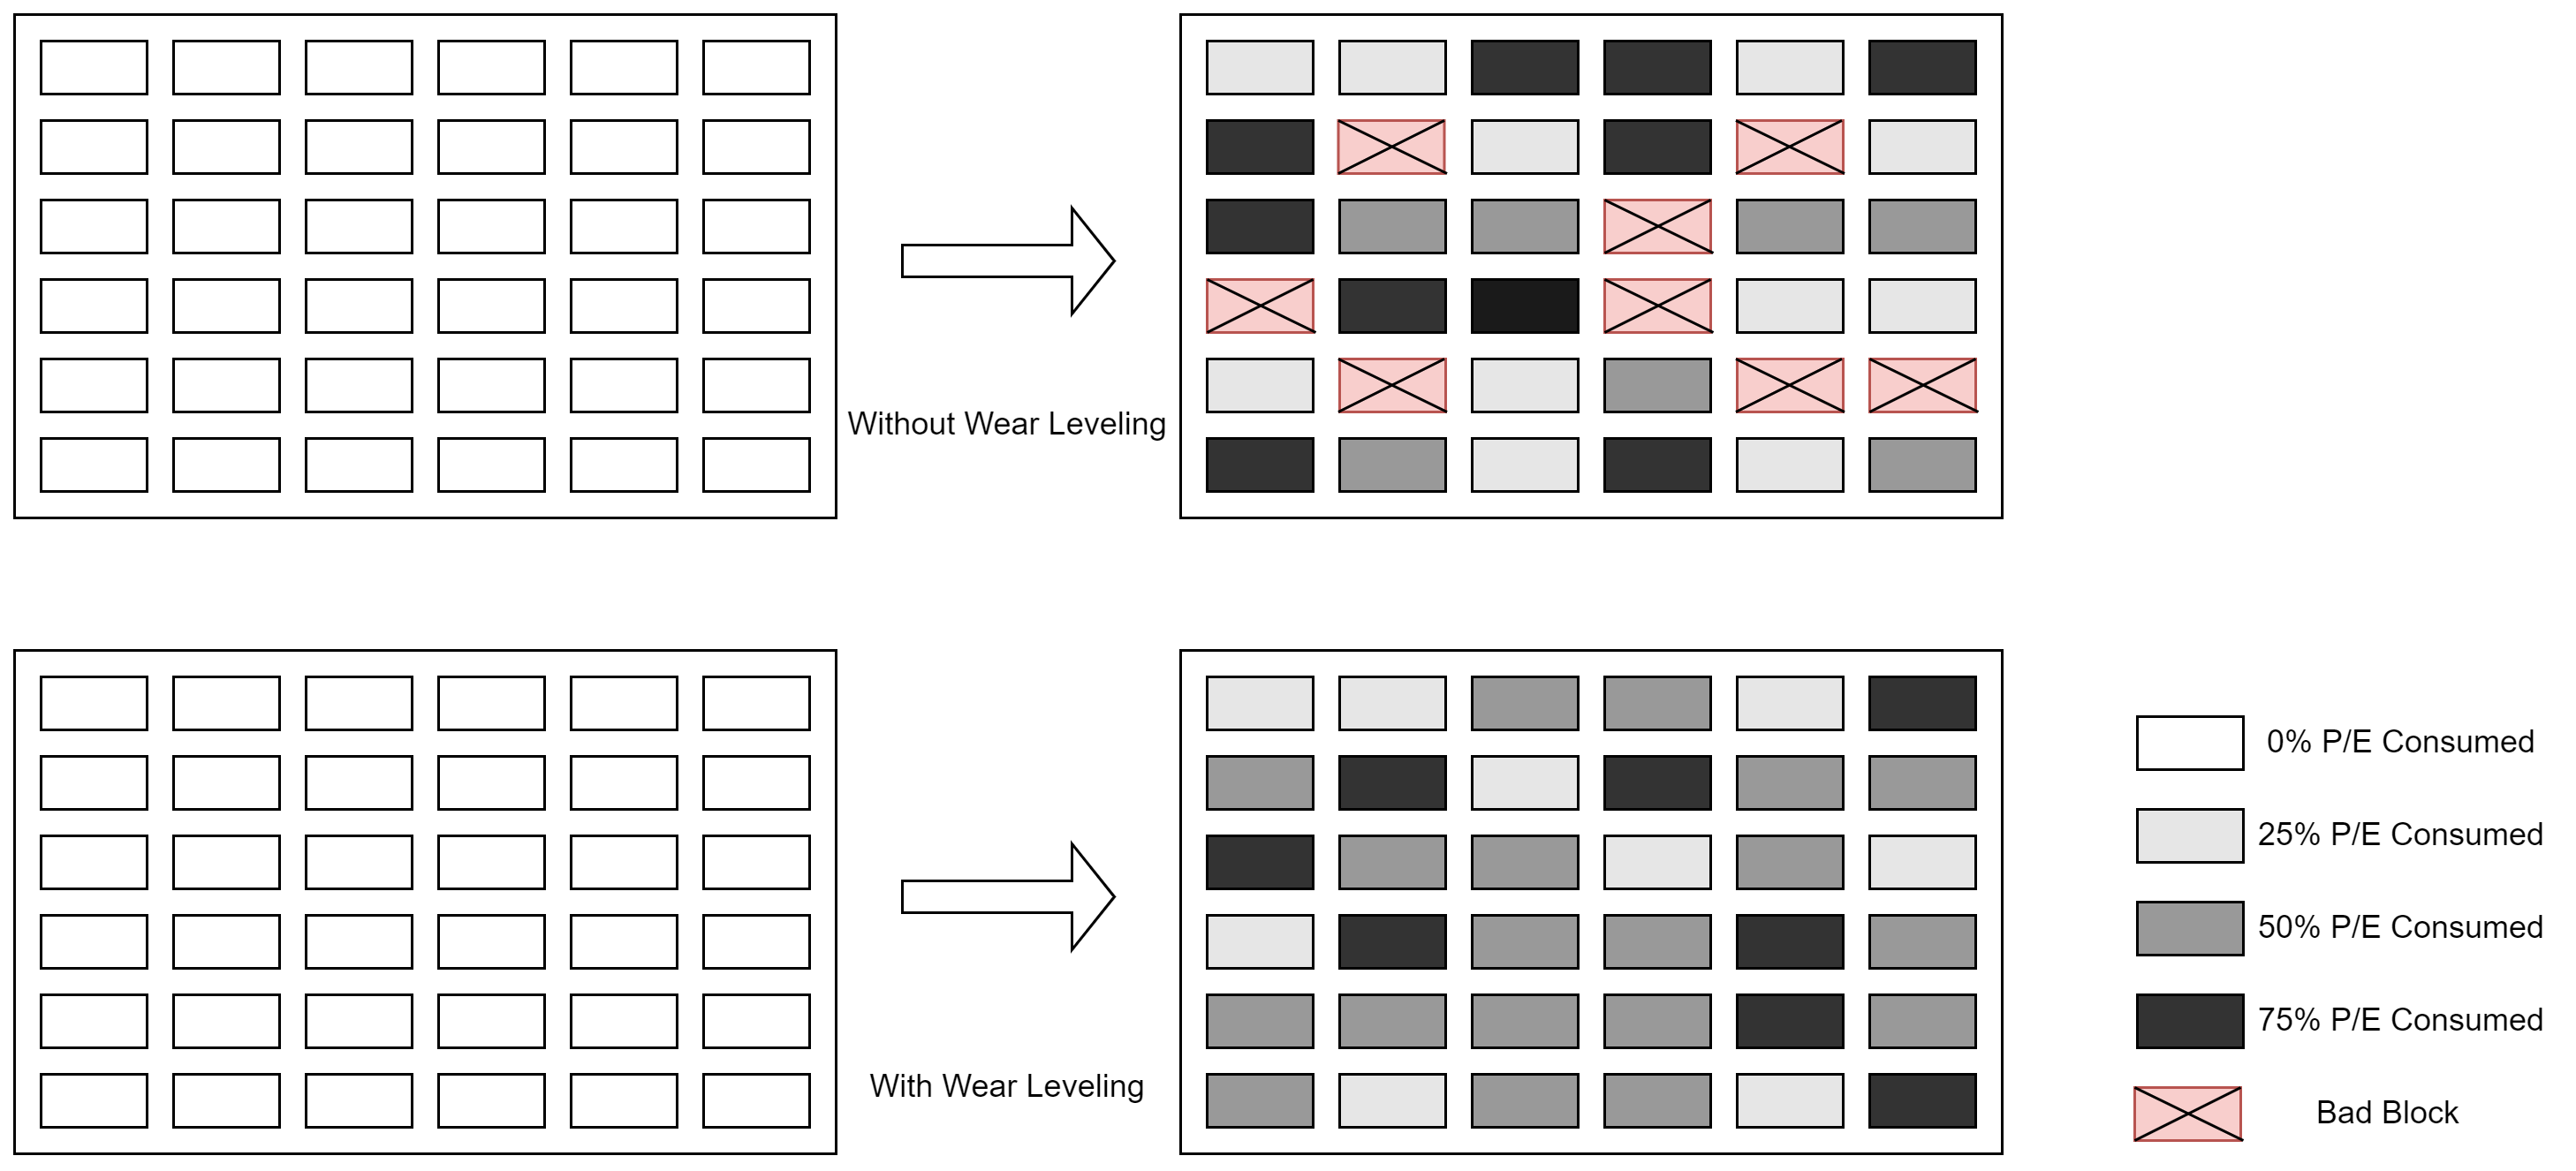
\includegraphics[width=1\textwidth]{picture/ch2/Wear_Leveling.png}
    \caption{Wear Leveling\cite{Wear_Leveling_Pic}}
    \label{f2.5}
\end{figure}

\subsection{Mapping Table}\label{s2.2.2}
\indent
由於\ref{s2.1.3}節所提到的 Erase Before Write 問題,因此 SSD 會先將接收到的資料暫存,之後寫入至其他區域,這樣可以減少寫入的延遲;同時為了讓 Host 覺得使用 SSD 與傳統硬碟的方式一致,所以增加轉換表,紀錄 Host 傳給 SSD 的 Logical Address 所對應的實際 Physical Address(如圖\ref{f2.6}所示)。通常會跟 \ref{s2.2.1} 所提到的 Wear Leveling 結合。\cite{5496970}
\begin{figure}[H]
    \centering
    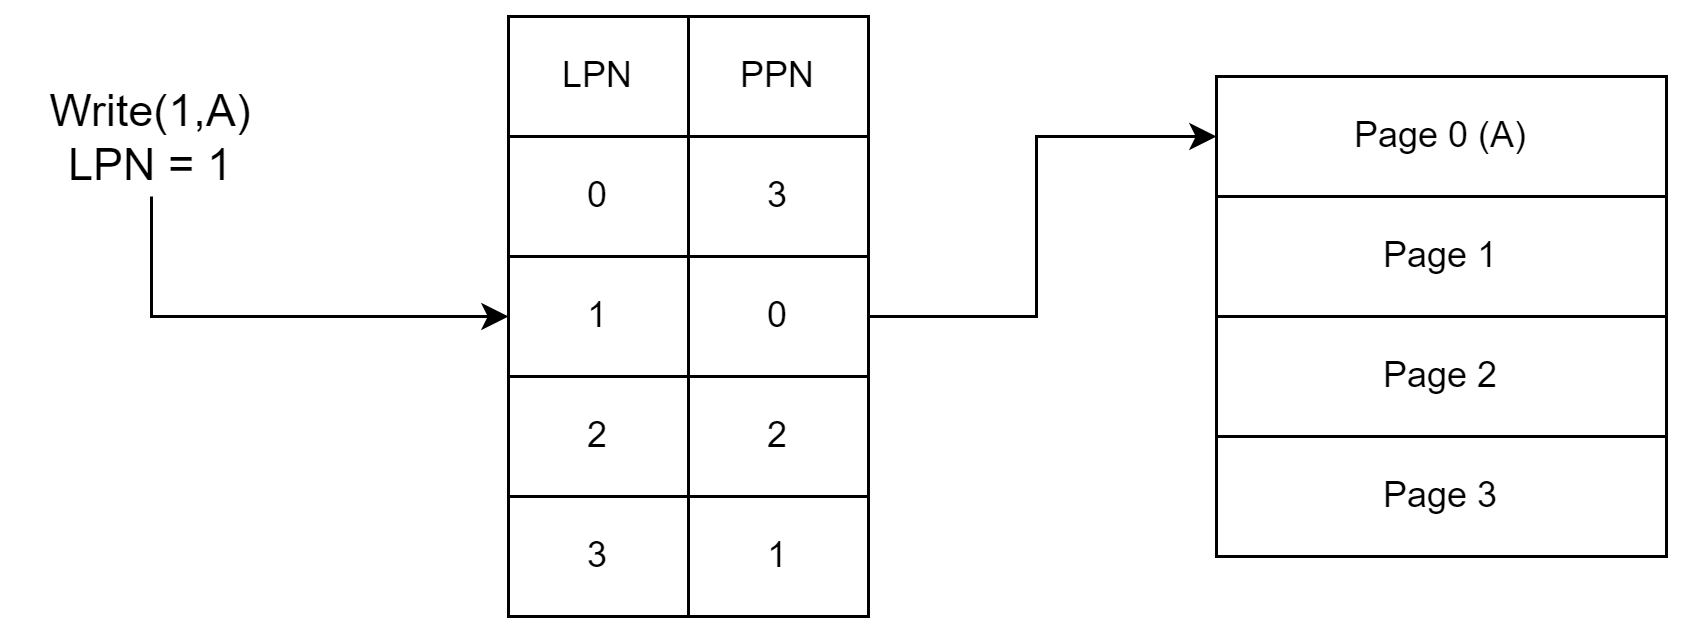
\includegraphics[width=1\textwidth]{picture/ch2/mapping_table.png}
    \caption{Mapping Table\cite{Mapping_Table}}
    \label{f2.6}
\end{figure}

\subsection{Garbage Collection}\label{s2.2.3}
\indent
由於\ref{s2.2.2}節所提到的功能,將資料寫到別的位置時,原本位置的 Block 就會有某些資料被視為無效,但還是有些資料是有效的,這時候就需要讀出來放到其他 Block 裡面,才可以將原本位置的 Block 清空,繼續作為空的 Block 寫入(如圖\ref{f2.7}所示)。由於清除資料時的延遲較高,FTL 通常都會挑選比較空閒的時候才執行這些搬移、清空資料的動作。\cite{BUX20101172}
\begin{figure}[H]
    \centering
    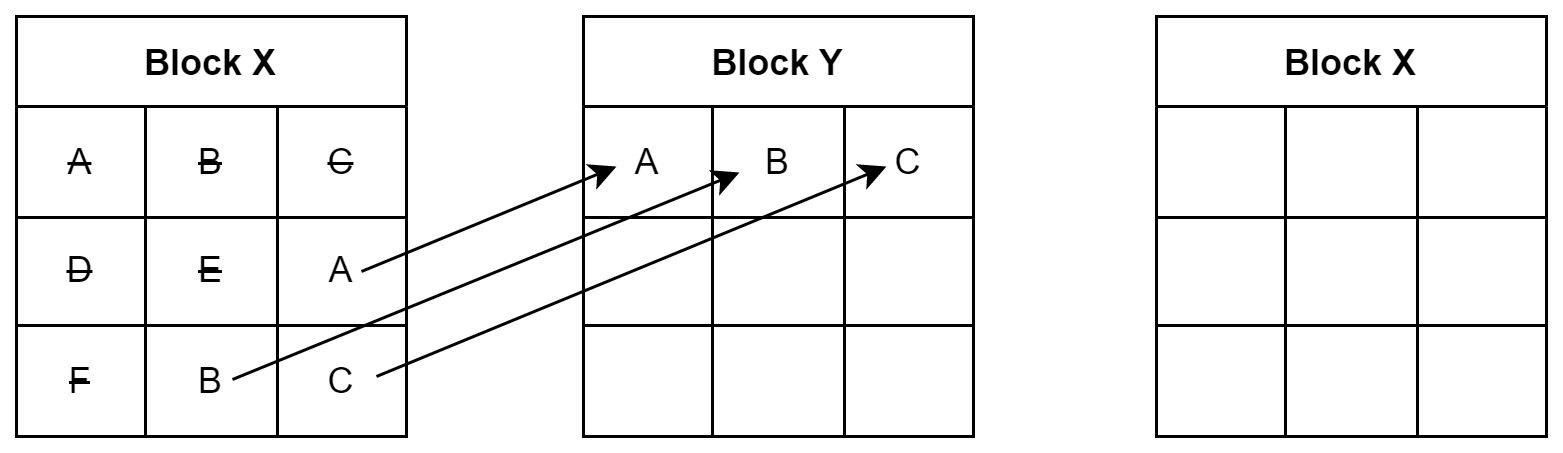
\includegraphics[width=1\textwidth]{picture/ch2/garbage_collection.png}
    \caption{Garbage Collection\cite{Garbage_Collection}}
    \label{f2.7}
\end{figure}

\section{Open-Channel SSD}\label{s2.3}
\indent
雖然 SSD 已經有了上述技術來管理以及延長壽命,不過這些功能都位於 SSD 內部的 FTL,Host 不知道這些資訊。而在雙方沒有溝通的狀況下,SSD 其實不知道 Host 需要的資料是什麼,容易造成重複讀取或是效率下降的問題,例如 SSD 可能會 Caching 到 Host 不需要的資料等問題。
而 Open-Channel SSD 開啟了一個可以利用 Host 資訊增進存取效能的可能性。\\
這種SSD將下列三種功能交給 Host 管理(如圖\ref{f2.8}所示):
%雖然 SSD 已經有了上述技術來管理以及延長壽命,不過由於這些技術仰賴於 SSD 內部的控制器及韌體管理,Host 完全不知情,所以寫入及讀取的延遲時間取決於韌體以及SSD控制器的穩定度,而為了讓延遲時間能夠掌控在 Host 的手上,也同時為了降低成本,於是有了Open Channel SSD。Open Channle SSD 將下列技術往上交給 Host 管理。
\begin{itemize}
    \item Mapping Table
    \item Garbage Collection
    \item 部分的 Wear Leveling
\end{itemize}
\begin{figure}[H]
    \centering
    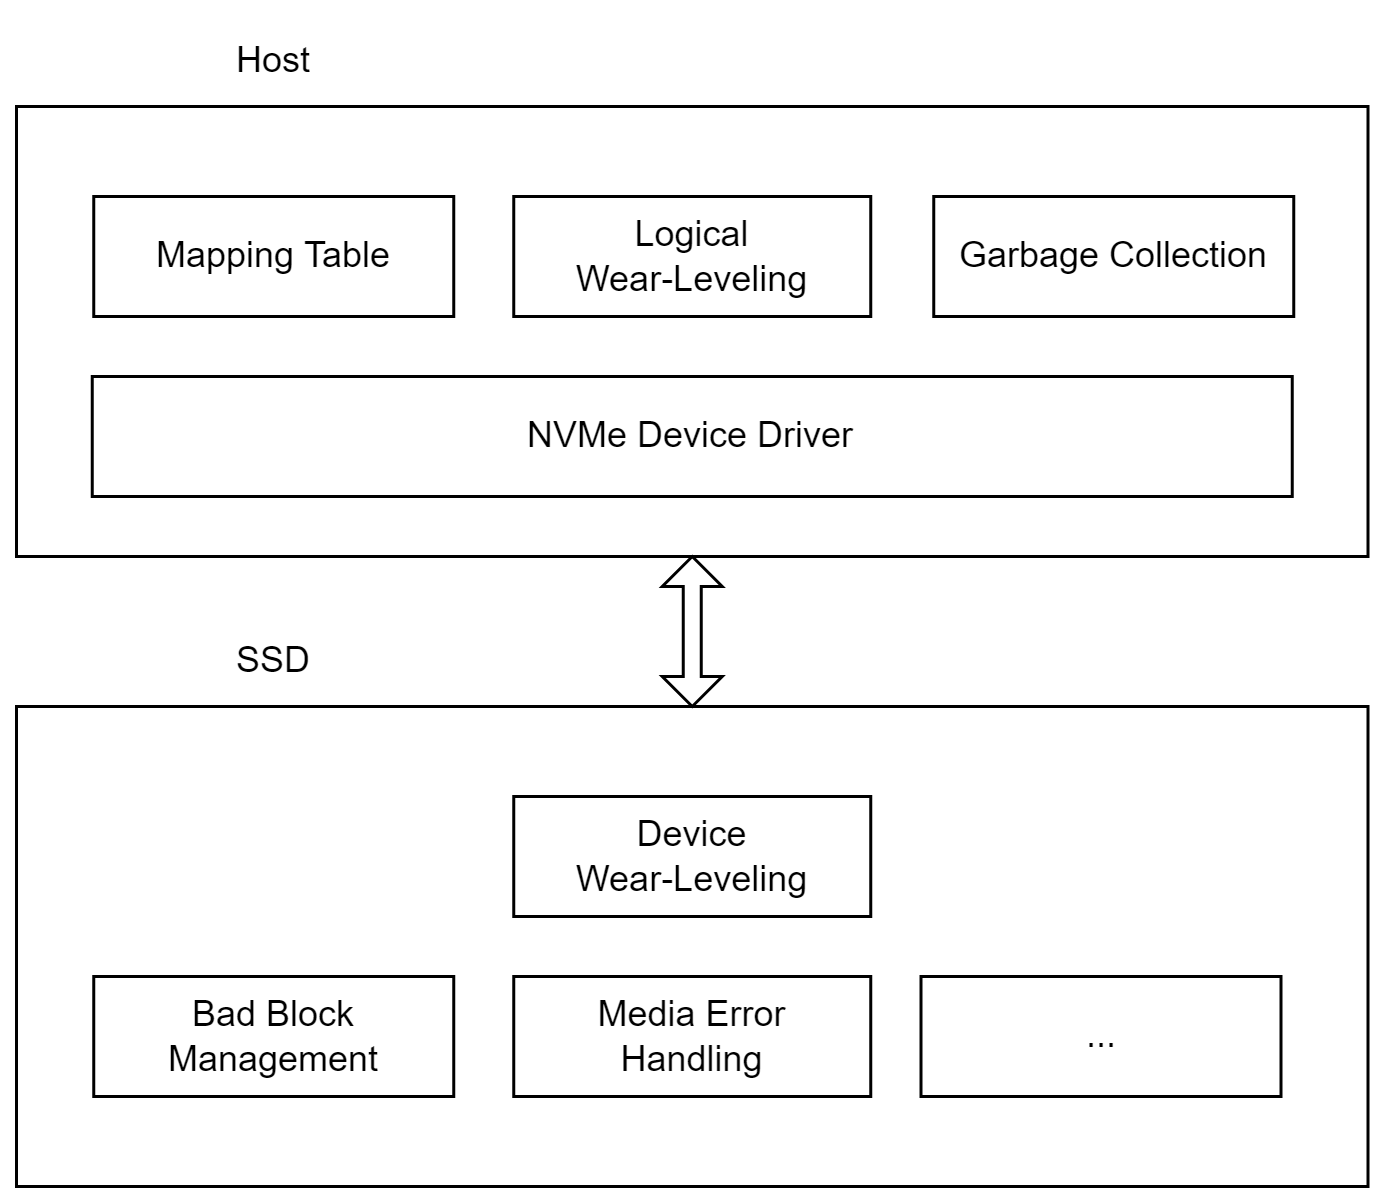
\includegraphics[width=1\textwidth]{picture/ch2/OPSSD.png}
    \caption{Open Channel SSD\cite{OPSSD}}
    \label{f2.8}
\end{figure}

\section{LightNVM}\label{s2.4}
\indent
LightNVM 是 Linux 之中用來管理 Open Channel SSD 的一個 Kernel Module,來實作上述交給 Host 管理的功能,可讓 Linux 系統正確辨識並能夠用控制一般SSD的方式對 Open Channel SSD 提出讀取、寫入、刪除等要求。本論文也是修改此模組來實作我們所需的功能。

\subsection{Line}\label{s2.4.1}
\indent
一般來說,SSD 內部的大小單位可以分為下列幾種,由大而小依序為:
\begin{itemize}
    \item Channel
    \item Lun
    \item Block
    \item Page
\end{itemize}
而 Line 會由每個 Lun 之中的一個 Block 所組成,如圖\ref{f2.9}所示。而在 LightNVM 之中,寫入以及 Garbage Collection 均採用此單位作為管理的主要架構,本論文提出的修改部分也與此有關。
\begin{figure}[H]
    \centering
    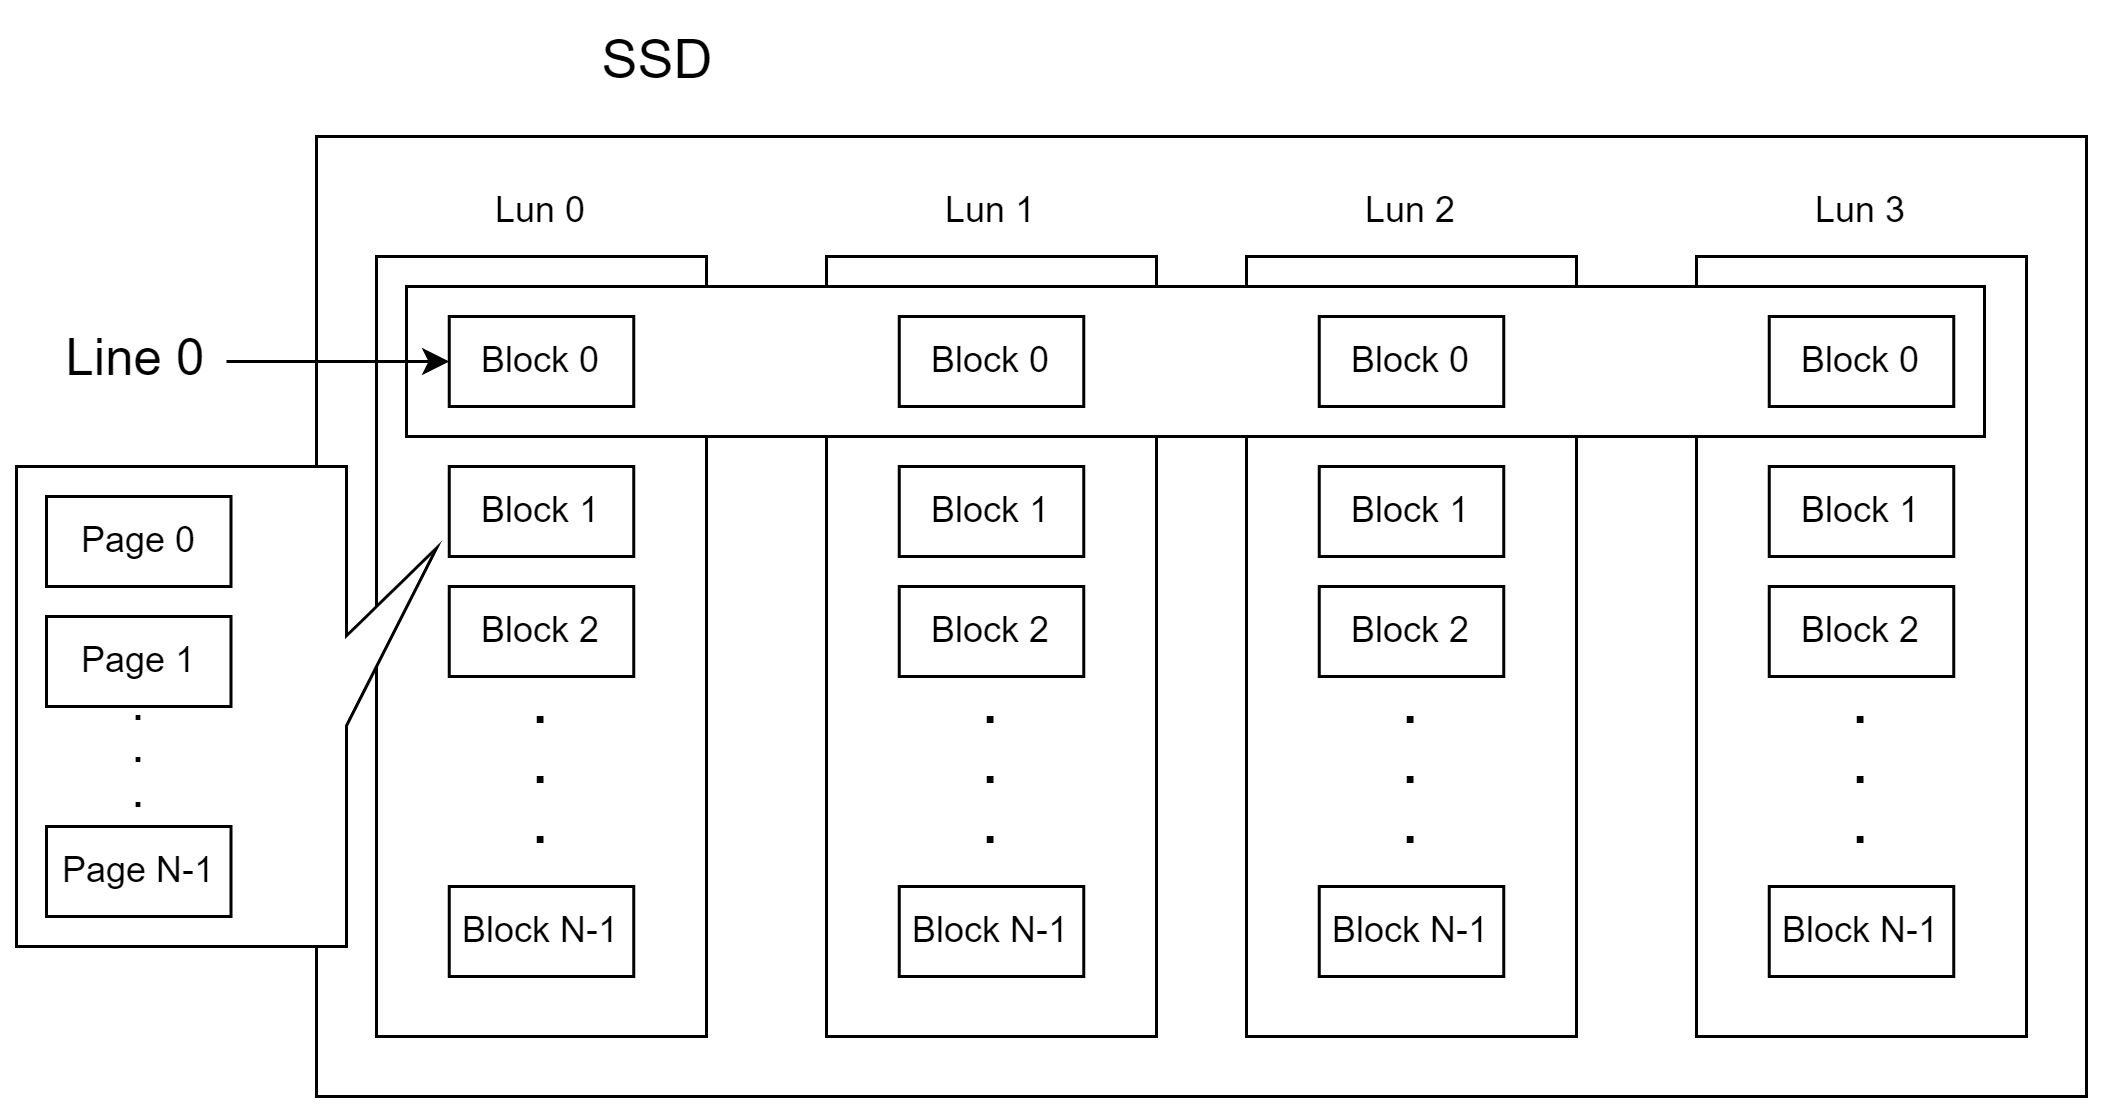
\includegraphics[width=1\textwidth]{picture/ch2/Line.png}
    \caption{單位大小}
    \label{f2.9}
\end{figure}